\documentclass{standalone}
\usepackage{tikz,ctex}
\usepackage{tikz-3dplot} % 2-1
\usepackage{unicode-math} % 2-5,4-1,4-2
\setmathfont{Fira Math Regular}
\setmainfont{Fira Sans}
\definecolor{background}{RGB}{239, 239, 239} % 4-5,6-2,6-5
\begin{document}
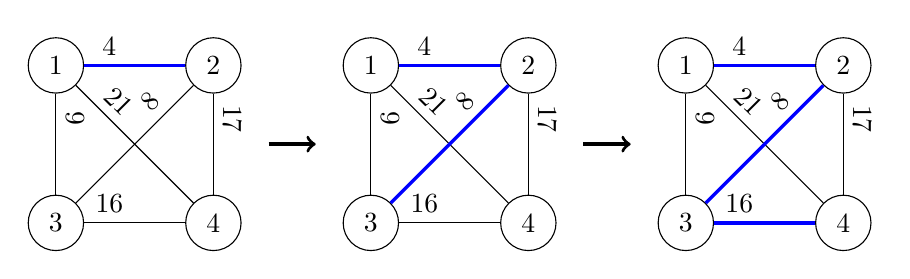
\begin{tikzpicture}
\foreach \n in {0,1,2}{
    \foreach \x/\y[count=\i] in {0/2,2/2,0/0,2/0}{
        \node[circle,minimum size=20pt,draw](\i\n) at (\x+4*\n,\y){\i};}
    \foreach \u/\v/\w in{1/2/4,1/3/9,1/4/21,2/3/8,2/4/17,3/4/16}{
        \draw (\u\n) -- (\v\n) node[near start,sloped,above] {\w};}}
\draw[->,very thick] (2.7,1)--(3.3,1);
\draw[->,very thick] (6.7,1)--(7.3,1);
\foreach \u/\v in{10/20,11/21,21/31,12/22,22/32,32/42}{
    \draw [very thick,blue] (\u) --(\v);}
\end{tikzpicture}
\end{document}